\documentclass[A4, landscape] {article}
\usepackage{tikz}
\usepackage{amsmath}
\usepackage{esvect}
\begin{document}

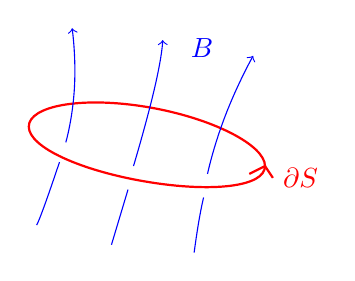
\begin{tikzpicture}
\draw [red, thick] plot [smooth cycle, tension=1] coordinates {(0,0) (1.5,-.7) (3,-.5) (1.5,.25)};
\draw [red,thick] (2.8,-.6)--(3,-.5)--(3.1,-.65) node[right] {$\textcolor{red}{\partial S}$};
\node at (2.2,1) {$\textcolor{blue}{\vv B}$};

\draw [blue] plot [smooth, tension=1] coordinates {(.1,-1.25) (.2,-1) (.39,-.45)};
\draw [blue, ->] plot [smooth, tension=1] coordinates {(.47,-.2)(.58,.5) (.55,1.25)};

\draw [blue] plot [smooth, tension=1] coordinates {(1.05,-1.5) (1.2,-1) (1.26,-.8)};
\draw [blue,->] plot [smooth, tension=1] coordinates {(1.33,-.5) (1.6,.5) (1.7,1.1)};

\draw [blue] plot [smooth, tension=1] coordinates {(2.1,-1.6) (2.16,-1.2) (2.22,-.9)};
\draw [blue,->] plot [smooth, tension=1] coordinates {(2.27,-.6) (2.5,.15) (2.85,0.9)};
\end{tikzpicture}

\end{document}